\documentclass[a4paper,titlepage]{scrartcl}
\pagestyle{plain}
\usepackage[utf8]{inputenc}
\usepackage[T1]{fontenc}
\usepackage[german]{babel}
\usepackage{float}
\usepackage{graphicx}
\usepackage{amsmath,amssymb,amstext}
\usepackage{enumerate}
\usepackage{units}

\numberwithin{equation}{section}

\title{Versuch P2-23: Laser B\\Vorbereitung}
\author{Gruppe Di-22\\Jonas Müller, Genti Saliu}
\date{08. Mai 2014}

\begin{document}
	\begin{titlepage}
		\maketitle
		\thispagestyle{empty}
	\end{titlepage}
	
\newpage
\pagenumbering{roman}
\tableofcontents

\newpage
\pagenumbering{arabic}

\section{Grundlagen}
\subsection{Kohärenzlänge}
Die Kohärenzlänge ist der maximale Weglängen- oder Laufzeitunterschied, den zwei Lichtstrahlen aus derselben Quelle haben dürfen, damit bei ihrer Überlagerung noch ein (räumlich und zeitlich) stabiles Interferenzmuster entsteht. Die Kohärenzlänge resultiert aus der zeitlichen Kohärenz und entspricht der optischen Weglänge, die das Licht während der Kohärenzzeit zurücklegt. Anders ausgedrückt, versteht man unter Kohärenzlänge die Entfernung, bis zu der man die Positionen der Nulldurchgänge im Wellenfeld noch sicher vorhersagen kann, wenn man den Abstand zweier benachbarter Nulldurchgänge kennt. 
\subsection{Interferenz und Beugung}
Interferenz beschreibt die Überlagerung von zwei oder mehr Wellen nach dem Superpositionsprinzip. Löschen sich die Wellen dabei gegenseitig aus, spricht man von \emph{destruktiver} Interferenz, bei Verstärkung der Amplited spricht man von \emph{konstruktiver} Interferenz. Das Muster aus Stellen konstruktiver und destruktiver Interferenz wird als Interferenzmuster bezeichnet. Im experimentellen Aufbau treten abwechselnd charakteristische Interferenzmaxima und Interferenzminima auf.\\ \\
Die Beugung oder Diffraktion ist die Ablenkung von Wellen an einem Hindernis. Durch Beugung kann sich eine Welle in den Raumbereichen ausbreiten, die auf rein geradem Weg durch das Hindernis versperrt wären. Zur Beugung kommt es durch Entstehung neuer Wellen entlang einer Wellenfront gemäß dem huygens-fresnelschen Prinzip. Diese können durch Überlagerung zu Interferenzerscheinungen führen.
\subsection{Laser}
Ein Laser (Light Amplification by Stimulated Emission of Radiation, auf Deutsch „Lichtverstärkung durch stimulierte Emission von Strahlung“) besteht konzeptionell aus drei Bestandteilen:
\begin{itemize}
\item Aktives Medium (Lasermedium) - Im aktiven Medium entstehen durch den optischen Übergang angeregter Atome oder Moleküle in einen energetisch günstigeren Zustand Photonen. Dabei ändert sich das Energieniveau eines Elektrons in einem Atom oder Molekül und es werden Photone freigesetzt. Das Medium kann gasförmig, flüssig oder fest sein.
\item Pumpe - Durch Einführen von Energie in das Lasermedium wird eine Besetzungsinversion erzeugt. In einem Medium mit nur zwei Energieniveaus sind im thermodynamischen Gleichgewicht Zustände geringer Energie mit höherer Wahrscheinlichkeit besetzt als Zustände höherer Energie. Die Inversion kann erzeugt werden, wenn das Medium mehr als 2 Niveaus und unterschiedliche Lebensdauern der angeregten Niveaus hat. Durch das Hineinpumpen (engl. pumping) von Energie in das Lasermedium wird dieses aus seinem thermodynamischen Gleichgewicht geholt, und es kann eine Inversion entstehen. Das Pumpen kann optisch (Einstrahlung von Licht) oder elektrisch (z. B. Gasentladung, elektrischer Strom bei Laserdioden) die Atome oder Moleküle des Lasermediums in angeregte Zustände bringen.
\item Resonator (Modenselektion) - Ein Resonator sorgt dafür, dass alle Photonen, die im Lasermedium entstehen, bis auf die in Impuls und Energie vom Resonator bevorzugten Photonen den Laser verlassen. Die Selektion des Resonators bewirkt, dass nur Photonen mit gleicher Energie und gleichem Impuls in das Lasermedium zurückgekoppelt werden. Über den Effekt der stimulierten Emission werden im besetzungsinvertierten Lasermedium von den zurückgekoppelten Photonen verstärkt Photonen mit ebenfalls gleicher Energie und gleichem Impuls erzeugt. Dies ist der Grund für die starke Kohärenz und Einfarbigkeit von Laserlicht.
\end{itemize}
Zunächst werden Atome im Lasermedium durch die eingespeiste Leistung von unteren Energieniveaus (z. B. Grundzustand) in energetisch höhere, d.h. angeregte Zustände versetzt. Dabei soll die mittlere Zerfallszeit der angeregten Zustände (in der Regel durch spontane Emission) möglichst lang sein. Somit bleibt die Pumpenergie dort „längere“ Zeit gespeichert, sodass eine Besetzungsinversion aufgebaut werden kann. Nun genügt eine Stimulierung eines Atoms durch ein Photon mit der auszustrahlenden Energie, damit das angeregte Atom wieder in seinen Grundzustand zurückfällt und dabei ein Photon der identischen Energie (also identischer Wellenlänge und Frequenz) sowie identischer Phasenlage wie das stimulierende Photon aussendet. Beide Photonen bewegen sich in die gleiche Richtung. Durch diese Verdoppelung des stimulierenden Photons wirkt das Lasermedium wie ein Lichtverstärker. Das „frisch entstandene“ zweite Photon kann dann seinerseits andere angeregte Atome zur Ausstrahlung stimulieren, und es kommt zu einer Kettenreaktion.\\ \\
Zu dieser Verstärkerwirkung kommt dann noch hinzu, dass sich die Anordnung in einem Resonator (s. u. bei Laserresonator) befindet, der durch seine Abmessungen auf die gewünschte Wellenlänge abgestimmt ist. So hat ein Photon bei mehrfachem Durchlaufen des Lasermediums genügend Chancen, andere Atome zu stimulieren. Der Resonator ist im Prinzip aus zwei Spiegeln an den Enden der Anordnung gebildet. Durch diese Spiegel wird auch die Richtung des erzeugten Lichtstrahls endgültig festgelegt. Einer der beiden Spiegel ist teildurchlässig ausgeführt, so dass ein Teil des Lichts austreten und seiner Nutzung zugeführt werden kann.
\subsection{Fouriertransformation}
Die Fourier-Transformation ist eine Methode der Fourier-Analysis, die es erlaubt, kontinuierliche, aperiodische Signale in ein kontinuierliches Spektrum zu zerlegen. Falls $f(t)$ eine integrierbare Funktion ist, so lautet ihre Fourier-Transformierte $F(\omega)$:
\begin{equation*}
F(\omega)=\frac{1}{2 \pi} \int^{+\infty}_{-\infty} f(t) e^{i \omega t} \, dt
\end{equation*}
Für die Rücktransformation gilt:
\begin{equation*}
f(t)=\frac{1}{2 \pi} \int^{+\infty}_{-\infty} F(\omega) e^{-i \omega t} \, dt
\end{equation*}
Das Beugungsbild, das entsteht, wenn kohärentes Licht durch einen Spalt auf einen Schirm fällt, kann durch die Fouriertransformierte der transmittierenden Welle $E(x, y)$ beschrieben werden.
\subsection{Michelson-Interferometer}
Das Verwendungsspektrum des Michelson-Interferometers ist sehr breit, wir werden ihn aber in dieser Versuchsreihe für sehr präzise Längenmessungen nutzen.\\ \\
Das Interferometer teil eine Lichtwelle in zwei Teile auf. Die zwei Wellen durchlaufen unterschiedlich lange Strecken oder Medien, in denen die Lichtgeschwindigkeit verschieden ist. Daraus ergibt sich eine Phasenverschiebung zwischen den zwei Wellen. Werden diese dann wieder zusammengeführt, kommt es zur Interferenz.
\begin{figure}[H]
	\centering
	\begin{tabular}{@{}r@{}}
		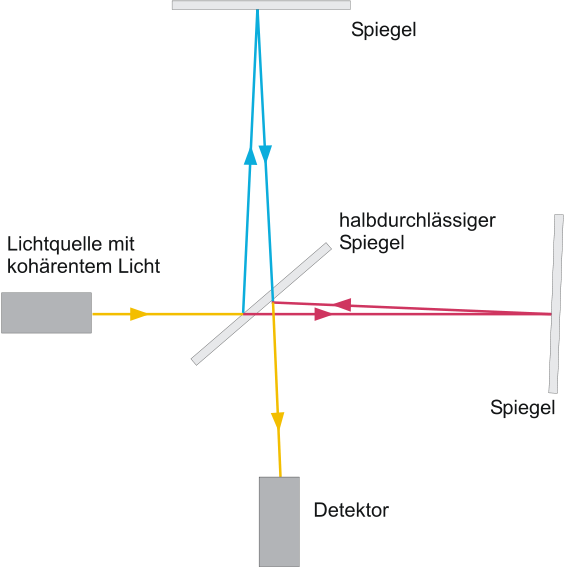
\includegraphics[width=0.6\textwidth]{Bilder/michelson.png}\\
		\footnotesize\sffamily\textbf{Quelle:} Wikipedia \cite{wiki:michelson}
	\end{tabular}
	\caption{Aufbau des Michelson-Interferometers}
	\label{fig:michelson}
\end{figure}
Die Aufteilung der Lichtwelle geschieht mittels eins halbdurchlässigen Spiegels. Dabei wird ein Teil der Lichtwellen durchgelassen, ein anderes Teil wird um $\unit[90]{Grad}$ reflektiert. Durchgelassene und reflektierte Wellen treffen auf einen vollständig reflektierenden Spiegel und werden wieder auf den halbdurchlässigen Spiegel zurückgeworfen. Wiederum wird ein Teil der Wellen reflektiert und ein anderes durchgelassen. Hinter dem halbdurchlässigen Spiegel überlagern sich die zwei Wellen und es kommt zur Interferenz.\\ \\
Die Phasen der beiden Wellen kann man durch Verschiebung einer der beiden Spiegel oder Änderung des Brechungsindexes des Mediums verschieben.\\
Sind die Wellen in Phase, so addiert sich ihre Amplitude (konstruktive Interferenz), sind sie gegenphasig, löschen sie sich gegenseitig aus (destruktive Interferenz).\\ \\
Über die Intensitätsmessung der resultieren Welle können auch kleinste Veränderungen des Gangunterschieds zwischen den beiden Wellen gemessen werden.\\ \\
Für den Gangunterschied $\Delta s$ gilt bei destruktiver Interferenz:
\begin{equation*}
\Delta s = m \cdot \lambda \quad \text{wobei} \quad m=1,2,...,n
\end{equation*}
und bei konstruktiver Interferenz:
\begin{equation*}
\Delta s = \frac{(2m - 1) \cdot \lambda}{2}
\end{equation*}
Aus dem Gangunterschied erhält man die Strecke $d$, bei dem ein Spiegel verschoben wurde, um den Phasenunterschied zu bewirken:
\begin{equation*}
\Delta s = 2 \cdot (S_1 - (S_2 + d))
\end{equation*}
mit $m$ die Anzahl der Hell-Dunkel-Durchgänge, $S_1$ und $S_2$ jeweils den Abstand der beiden Spiegel vom Mittelpunkt des halbdurchlässigen Spiegels.
\subsection{Dopplereffekt}
Der Doppler-Effekt ist die zeitliche Stauchung bzw. Dehnung eines Signals bei Veränderungen des Abstands zwischen Sender und Empfänger während der Dauer des Signals. Ursache ist die Veränderung der Laufzeit. Dieser Effekt kann bei allen Arten von Wellen beobachtet werden.
\begin{itemize}
\item Beobachter in Ruhe, Signalquelle bewegt\\ \begin{equation*}
f_B=\frac{f_S}{1 - \frac{v}{c}}
\end{equation*}
\item Beobachter bewegt, Signalquelle in Ruhe\\ \begin{equation*}
f_B=f_S \left(1 - \frac{v}{c}\right)
\end{equation*}
\item Beobachter und Signalquelle bewegt\\ \begin{enumerate}
\item Sender und Empfänger bewegen sich aufeinander zu \begin{equation*}
f_B=f_S \cdot \frac{c + v_B}{c - v_S}
\end{equation*}
\item Sender und Empfänger bewegen sich voneinander weg
\begin{equation*}
f_B=f_S \cdot \frac{c - v_B}{c + v_S}
\end{equation*}
\end{enumerate}
\end{itemize}
$f_S$ - Grundfrequenz der Welle\\
$c$ - Ausbreitungsgeschwindigkeit der Welle\\
$v$ - Geschwindigkeit der Wellenquelle bzw. Beobachters\\
$v_B$ - Geschwindigkeit des Beobachters \\
$v_S$ - Geschwindigkeit des Senders der Wellen relativ zum Medium
\newpage
\section{Spaltversuch}
Dieser Versuch hat demonstrativen Effekt. Es soll gezeigt werden, dass die Beugungsfigur eines Spaltes der Fouriertransformierten des Spaltbildes entspricht.\\ \\
Dazu wird die Intensität der Beugungsfigur mit einem Phototransistor gemessen und mithilfe des FFT-Programms im Rechner ein Spaltbild gewonnen. Es ist nicht zu erwarten, dass das zurückgewonnene Spaltbild genau dem Originalspaltbild entspricht, weil bei der Fouriertransformation von Beugungsfiguren komplizierter Objekte Phaseninformation fehlt.
\section{Michelson-Interferometer}
\subsection{Bestimmung des Magnetostriktionskoeffizienten}
In diesem Versuch soll man mithilfe des Michelson-Interferometers die infolge eines angelegten magnetischen Feldes (Magnetostriktion) sehr gering zu erwartende Längenabhängigkeit vom Nickel überprüfen und die Bestimmung der Magnetostriktionskoeffizienten erfolgen.\\ \\
Zunächst umgeben wir den Ni-Stab mit einer stromdurchflossenen (beide Stromrichtungen, Strom kurz eingeschaltet, maximal $\unit[5]{A}$) Spule und setzen einen der Interfermoterspiegel auf seine Stirnfläche. Es ist dann anhand der im Interfermoter entstehenden Hell-Dunkel-Durchgängen möglich die Längenänderung des Stabs und daraus die magnetostriktive Konstante $\alpha$ zu bestimmen.\\ \\
Das vom Strom $I$ induzierte Magnetfeld einer Spule der Länge $L$ mit $n$ Windungen beträgt:
\begin{equation*}
H=\frac{n \cdot I}{L}
\end{equation*}
Ausserdem berechnet sich die magnetostriktive Konstante $\alpha$ aus der Längenänderung $\Delta l$ und der initialen Länge $l_0=L$:
\begin{equation*}
\alpha=\frac{\Delta l}{l_0}
\end{equation*}
Man erhält für $\Delta l$:
\begin{equation*}
\Delta l = \alpha L H = \alpha n I
\end{equation*}
Für Amplitudenmaxima gilt:
\begin{equation*}
m \cdot \frac{\lambda}{2}= \Delta l = \alpha n I \quad \Rightarrow \Delta l = \frac{m \lambda}{2n}=\alpha I
\end{equation*}
Für Minima:
\begin{equation*}
\frac{(2m-1) \cdot \lambda}{4}=\Delta l = \alpha n I \quad \Rightarrow \Delta l = \frac{(2m-1)\cdot \lambda}{4n}=\alpha I
\end{equation*}
Somit lässt sich $\alpha$ aus der Steigung der Ausgleichsgerade für die gemessene Werten für $\Delta l$ und Spulenstrom $I$ bestimmen.
\subsection{Wellenlänge des Laserlichts}
Nun soll man die Wellenlänge des Laserlichts bestimmen. Wir nutzen hierfür ein anderes Interferometer. Aus
\begin{equation*}
\Delta l = \lambda \frac{m}{2}
\end{equation*}
soll man mit Ausgleichsrechung die Wellenlänge $\lambda$ bestimmen.
\subsection{Demonstration des Dopplereffekts}
\subsubsection{Bei Lichtwellen mit $v \approx c$}
Es sollte jetzt der Dopplerfekt mit Lichtwellen gezeigt werden. Wir nutzen dafür ein (justiertes) Interferometer, indem wir einen seiner Spiegel mit einem Motor gleichmäßig mit Geschwindigkeit $v$ bewegen. Dieser Spiegel ist zunächst Empfänger und dann Sender, deshalb bildet sich dort eine Schwebung (Interferenz von Wellen). Laut obiger Einführung gilt dann für die Frequenzänderung (einmal Beobachter in Bewegung, Sender in Ruhe, dann Beobachter in Ruhe, Sender in Bewegung):
\begin{equation*}
\Delta f=f_S \cdot \frac{v_B + v_S}{c-v_S}
\end{equation*} 
Es gilt $v=v_B=v_S$:
\begin{equation*}
\Delta f = f \cdot \frac{2 \cdot v}{c - v}
\end{equation*}
$\Delta f$ soll durch Auszählen der Intensitätsschwankung mit einer Stoppuhr bestimmt werden. Daraus kann man die Spiegelgeschwindigkeit bestimmen:
\begin{equation*}
v=\frac{c}{1 + \frac{2}{\alpha}} = \frac{c}{1 + T \cdot f} \approx \frac{c}{T \cdot f} = \frac{\lambda}{T}
\end{equation*}
mit $T$ die Periodenlänge der Schwebung ($\Delta f = \frac{2}{\Delta T}$).\\ \\
Die über das Interferometer bestimmte Geschwindigkeit des Spiegels soll nun auch mit der sich aus direkten Messungen ergebende Geschwindigkeit verglichen werden:
\begin{equation*}
v=\frac{\Delta x}{\Delta t}
\end{equation*}
\subsubsection{Bei Schallwellen}
Es sollte eine schwingende Stimmgabel vom Ohr weg und dann auf das Ohr bewegt werden, mit und ohne reflektierende Wand in der Nähe.\\ \\
Bewegt sich die Gabel auf das Ohr zu, so soll ein steigend höherer Ton zu hören sein und umgekehrt. Ist eine reflektierene Wand in der Nähe, so überlagern sich Wellen mit verschiedenen Frequenzen, sie interferieren und bilden eine Schwebung.
\newpage
\section{Faraday-Effekt und Pockels-Effekt}
\subsection{Intensitätsmodulation anhand des Faraday-Effekts}
\subsection{Bestimmung der Verdetschen Konstante von Bleisilikatglas}
\subsection{Intensitätsmodulation anhand des Pockel-Effekts}
\subsection{Konstantenbestimmung $k=\Delta n(E)$ für $LiNbO_3$}
\newpage
\section{Optische Aktivität}
\subsection{Spezifisches optisches Drehvermögen einer Zuckerlösung}
\subsection{Spezifisches optisches Drehvermögen einer Sorboselösung}

\newpage
\bibliographystyle{plain}
\bibliography{quellen}

\end{document}